\section{Bancos de dados paralelos}

Bancos de dados paralelos ou massivamente paralelos (MPP, do inglês 
\emph{massively parallel processing}) também não são tecnologia 
recente, discussões sobre esse assunto e implementações de sistemas
datam da década de 80-90 \cite{Dewitt1992, Fushimi1986}. Nestes 
sistemas, os dados das tabelas são distribuídos em diversos 
nós de um cluster e o processamento de consulta é paralelizado.

Os dados podem ser distribuídos através de particionamento vertical,
onde as tabelas são quebradas por colunas; horizontal, onde as 
tabelas são quebradas por tuplas; ou ambos. A distribuição dos 
dados entre os nós pode utilizar o conhecimento prévio
das consultas mais utilizas no sistema (\emph{query workload}),
e o otimizador de consultas, nestes casos, conhecendo a forma
como os dados estão distribuídos, pode repassar a parte das
consultas para os nós específicos que devem processá-la. O problema
geral desta abordagem é que existe a possibilidade de desbalanceamento
de nós \emph{data skew}; e o particionamento por funções de hash é portanto também
bastante utilizado, pois através de boas funções de hash é possível
evitar este desbalanceamento..

A arquitetura dos bancos de dados paralelos pode ser de compartilhamento 
de memória (\emph{shared-memory}, onde a memória é compartilhada entre os
nós do cluster; compartilhamento de disco (\emph{shared-disk}), onde
cada nó do cluster possui sua própria memória, mas o disco é compartilhado
entre todos os nós; ou sem compartilhamento (\emph{shared-nothing}), onde
cada nó possui sua própria memória e disco e o compartilhamento de dados
entre nós do cluster se faz através de transferência por mensagens. As 
arquiteturas com compartilhamento (\emph{shared-memory} e \emph{shared-disk})
se mostraram ineficientes em escalabilidade para grandes implantações
\cite{Dewitt1992, Stonebraker1986}. A Figura \ref{fig:mpp_arq} mostra
um banco de dados paralelo com um nó mestre e arquitetura sem 
compartilhamento.


\begin{figure}
        \centering
        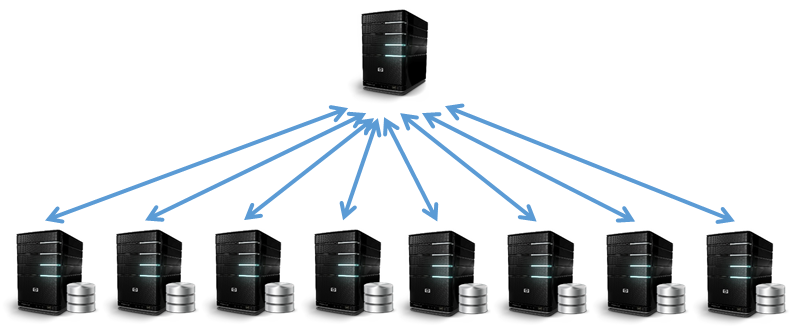
\includegraphics[width=\linewidth]{./mpp_database.png}
        \caption{Banco de dados paralelo e a arquitetura sem compartilhamento.}
        \label{fig:mpp_arq}
\end{figure}

Os operadores da álgebra relacional são todos paralelizáveis, principalmente
a junção, com algoritmos de espalhamento dos dados por função de hash 
\cite{Schneider1989}. A ideia principal destes algoritmos é a de que cada 
nó lê sua parcela dos dados, aplica uma função de hash nos atributos da
junção para determinar o nó de destino e envia os dados para os nós específicos.
Desta forma, quando os nós agora recebem os dados, há a garantia (pela
função de hash) de que os nós que irão participar do resultado da junção 
estão fisicamente localizados juntos, neste passo. Cada nó então executa um
algoritmo linear de junção, tipicamente uma junção por hash em memória,
e reporta o resultado para o nó coletor. Este processo é demonstrado na 
Figura \ref{fig:mpp_hashjoin}. Nesta figura, é mostrada uma arquitetura
com quatro nós sem compartilhamento, e estes quatro nós estão replicados 
em duas camadas para melhor mostrar a fase de espalhamento dos dados
por função de hash (\emph{shuffle}).

\begin{figure}
        \centering
        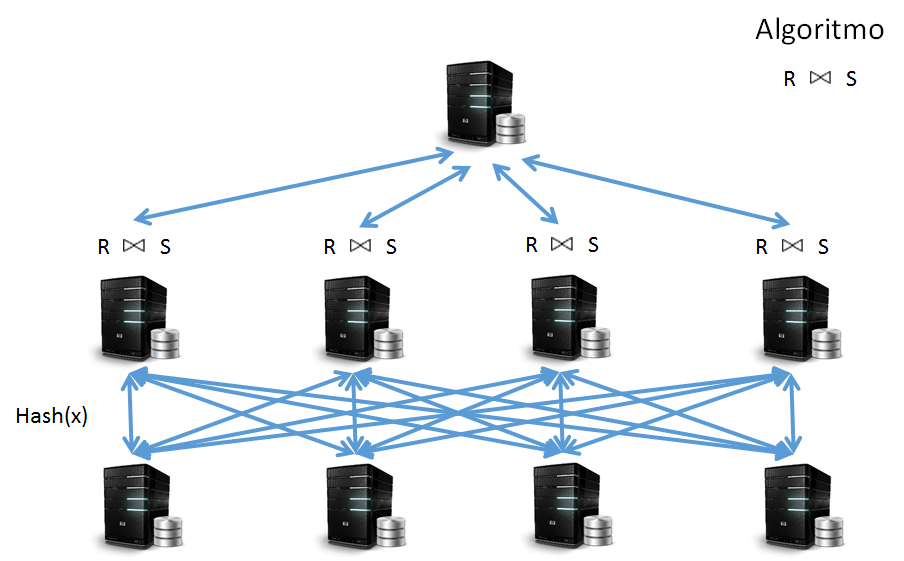
\includegraphics[width=\linewidth]{./mpp_hashjoin.png}
        \caption{Junção por hash em um banco de dados paralelo sem compartilhamento.}
        \label{fig:mpp_hashjoin}
\end{figure}

A solução do problema da contagem dos triângulos da Seção \ref{sec:triangulos} utilizando
banco de dados paralelos não envolve mistérios, uma vez que tal tecnologia 
implementa a álgebra relacional e já mostramos na Seção \ref{sec:relacional}
a consulta SQL que resolve o problema. Esta consulta envolve duas junções, 
que serão executadas em paralelo, e as seleções de remoção de duplicatas que
serão aplicadas após as junções no fluxo de execução das consultas (\emph{pipeline}).


